\documentclass[11pt,letterpaper]{article}
\usepackage[utf8]{inputenc}

%----- Configuración del estilo del documento------%
\usepackage{epsfig,graphicx}
\usepackage[left=2cm,right=2cm,top=1.8cm,bottom=2.3cm]{geometry}
\usepackage{fancyhdr}
\usepackage{lastpage}
\usepackage{url}
\pagestyle{fancy}
\fancyhf{}
\rfoot{\textit{Página \thepage \hspace{1pt} de \pageref{LastPage}}}


%------ Paquetes matemáticos básicos --------%
\usepackage{amsmath}
\usepackage{amssymb}
\usepackage{amsthm}
\usepackage{comment}

\usepackage[spanish]{babel}
\usepackage{graphicx}
\usepackage{hyperref}

\usepackage{tabularx}
\usepackage{xcolor}
\usepackage[table]{xcolor}
\usepackage{colortbl}
\usepackage{array, multirow, multicol, tabularx}
\usepackage{tcolorbox}
\newtheorem{theorem}{Theorem}[section]
\newtheorem{corollary}{Corollary}[theorem]
\newtheorem{lemma}[theorem]{Lemma}

%------si-------%
\definecolor{B}{HTML}{FFFFFF}
\definecolor{G}{HTML}{5e5e5e}
\definecolor{R2}{HTML}{d53d40}
\definecolor{A2}{HTML}{034190}
\definecolor{V2}{HTML}{7faa50}
\newcommand{\R}{\mathbb{R}}
\newcommand{\C}{\mathcal{C}}
\newcommand{\N}{\mathbb{N}}
\newcommand{\Z}{\mathbb{Z}}
\newcommand{\Q}{\mathbb{Q}}
\newcommand{\equalflipped}{\rotatebox[origin=c]{90}{$=$}}
\renewcommand{\theenumi}{\Roman{enumi}}
\renewcommand{\labelenumi}{{\theenumi}.}

\begin{document}

%------ Encabezado -------- %

\begin{center}
    \begin{minipage}{3cm}
    	\begin{center}
    		\includegraphics[height=3.4cm]{logo_unam.png}
    	\end{center}
    \end{minipage}\hfill
    \begin{minipage}{10cm}
    	\begin{center}
    	\textbf{\large Universidad Nacional Autónoma de México}\\[0.1cm]
        \textbf{Facultad de Ciencias}\\[0.1cm]
        \textbf{OMUM 2025}\\[0.1cm]
        Examen selectivo\\[0.1cm]
         El\'ias L\'opez Rivera\,\,Adolfo Angel Cardoso Vasquez$^{2}$\\[0.1cm]
        Fecha:\,\,16/07/2025
    	\end{center}
    \end{minipage}\hfill
    \begin{minipage}{3cm}
    	\begin{center}
    		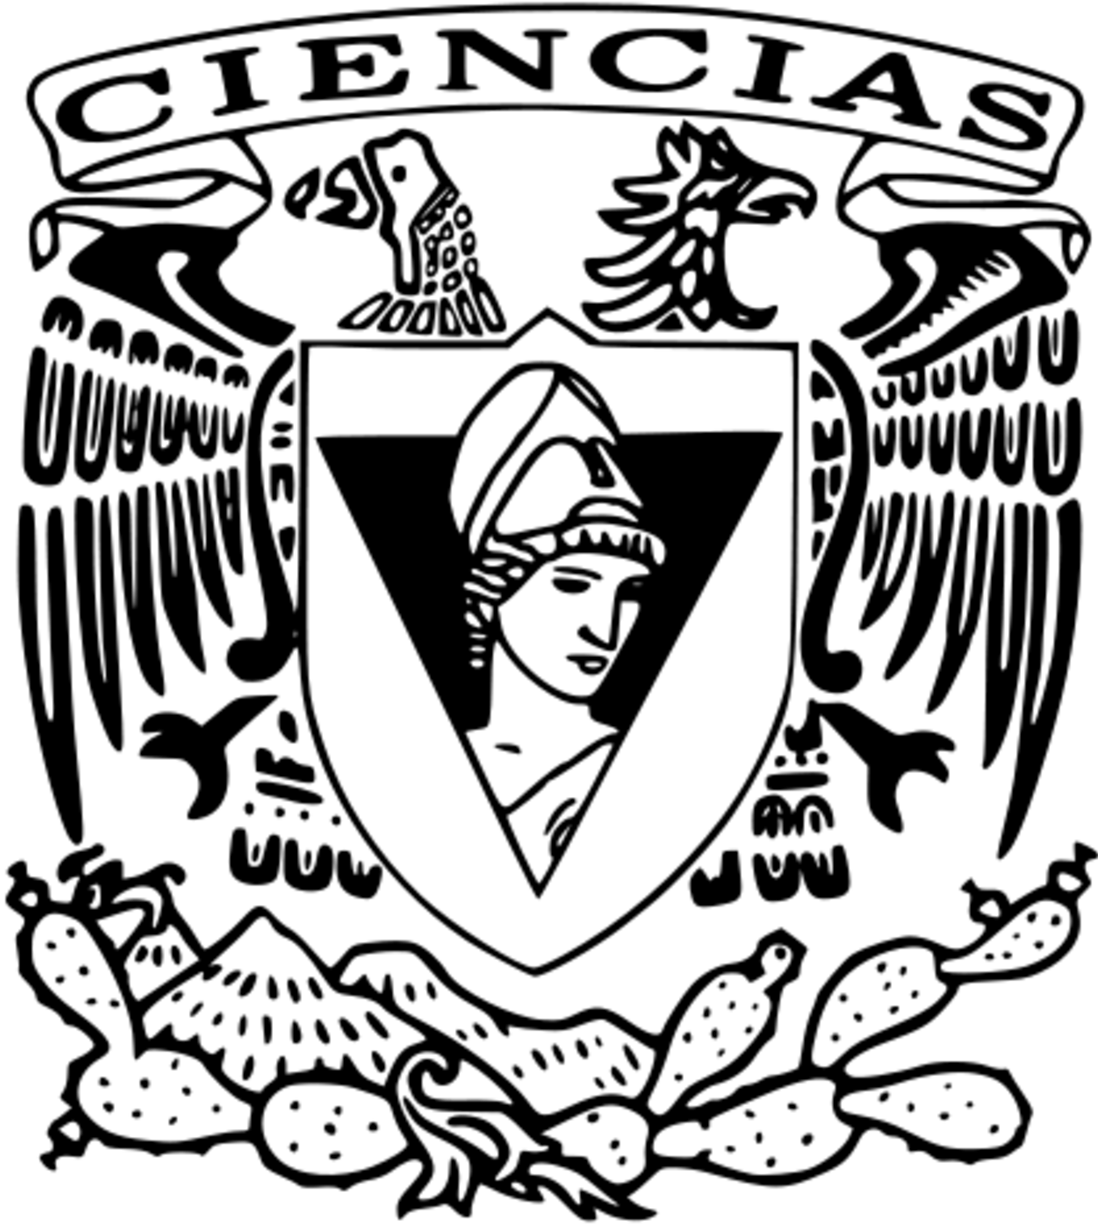
\includegraphics[height=3.4cm]{Logo_FC.png}
    	\end{center}
    \end{minipage}
\end{center}

\rule{17cm}{0.1mm}

%------ Fin de encabezado -------- %
\,\\
\begin{tcolorbox}[
	title = \textcolor{black}{\textcolor{white}{Problema 1}},]
\textit{ Para $n$ un n\'umero natural, consider $A_n:=\{1,2,\cdots,n\}$. Para $B\subset A_n$ se considera \\
$S_B=a_r-a_{r-1}+a_{r-2}-\cdots+(-1)^{r-1}a_1$, si $B=\{a_r>a_{r-1}>\cdots>a_1\}$, Calcula:
\begin{equation*}
    \sum_{B\subset A_n}\,S_B
\end{equation*}}
\end{tcolorbox}
\begin{proof}\,\\
    \,\\
Tomemos $k\in A_n$, queremos ver la contribuci\'on de $k$ en $\sum_{B\subset A_n}\,S_B$, para esto pensemos en la forma 
de un conjunto $B$ que contiene a $k$:\,\\
\begin{equation*}
    B=\{\underbrace{a_1,.....}_\text{valores\,$<k$},\,k\,,\underbrace{.....,a_r}_\text{valores\,$>k$}\}
\end{equation*}\,\\
Debido a las hip\'otesis del problema sabemos que la parte derecha del conjunto determinara el signo de $k$ en $S_B$, si hay una cantidad par su signo sera positivo y si hay una cantidad impar tendra signo negativo, ahora particionemos $A_n$ en dos conjuntos a partir de $k$,
$A_<:=\{n\in A_n|n\leq k\}$ y $A_>:=\{n\in A_n|n>k\}$, notemos que $B$ puede ser representado por la uni\'on de dos subconjuntos $B_1\subset A_<$ y $B_2\subset A_>$, notemos que es necesario que $k\in B_1$ mientras que $B_2$ puede ser cualquier subconjunto, hasta el vacio, la cantidad se subconjuntos $B_1$ de $A_<$ que contienen a $k$ es $2^{k-1}$, mientras que para 
$0\leq i\leq n-k$ la cantidad de subconjuntos con $i$ elementos de $A_>$ es $C^{n-k}_i$, por tanto la cantidad de subconjuntos que cumplen ambas condiciones es $2^{k-1}\,C^{n-k}_{i}$, por tanto la conribuci\'on total de $k$ en $\sum_{B\subset A_n}\,S_B$ es:
\begin{equation*}
    \sum_{i=0}^{n-k}\,(-1)^{i}\,k2^{k-1}\,C^{n-k}_{i}
\end{equation*}\,\\
Finalmente iteramos sobre todo $A_n$:\,\\
\begin{equation*}
    \sum_{B\subset A_n}\,S_B=\sum_{k=1}^n k\,\sum_{i=0}^{n-k}\,(-1)^{i}\,2^{k-1}\,C^{n-k}_{i}=\sum_{k=1}^{n}2^{k-1}\, \sum_{i=0}^{n-k}\,(-1)^{i}\,C^{n-k}_{i}
\end{equation*}\,\\
\,\\
Aplicando la identidad del binomio de Newton:\,\\
\,\\
\begin{equation*}
    \sum_{B\subset A_n}\,S_B=\sum_{k=1}^{n}k2^{k-1}(1-1)^{n-k}=n2^{n-1}
\end{equation*}
\end{proof}
\begin{tcolorbox}[
	title = \textcolor{black}{\textcolor{white}{Problema 2}},]
\textit{Sea $A:=\{n\in \N| n\,\,es \,\,compuesto\,\,potencia\,\,de \,\,un\,\,primo\}$, definamos $f(n)$ como el promedio de los divisores de $n\in A$.Demuestra que la siguiente suma converge\,\\
\begin{equation*}
    \sum_{n\in A}\,\frac{1}{f(n)}
\end{equation*}
}
\end{tcolorbox}
\begin{proof}\,\\
    \,\\
    Si $n\in A$ entonces $n=p^k$ con $k>1$, $k\in \N$ y $p$ un numero primo, por tanto:\,\\
    \,\\
    \begin{equation*}
        f(n)=\frac{\sum_{i=0}^k p^i}{k+1}=\frac{p^{k+1}-1}{(k+1)(p-1)}\implies \frac{1}{f(n)}=\frac{(k+1)(p-1)}{p^{k+1}-1}
    \end{equation*}\,\\
    \,\\
    Como $p>1\implies p^k>1\implies -1<-p^k\implies p^{k+1}-1<p^{k+1}-p^k\implies \frac{1}{p^{k+1}-1}<\frac{1}{p^k(p-1)}$ por tanto:\,\\
    \,\\
    \begin{equation*}
        \frac{1}{f(n)}<\frac{(k+1)(p-1)}{p^k(p-1)}=\frac{k+1}{p^k}
    \end{equation*}\,\\
    Luego tenemos que:\,\\
    \,\\
    \begin{equation*}
        \sum_{p\,\,\,primo}\,\sum_{k=2}^{\infty}\,\frac{(k+1)(p-1)}{p^{k+1}-1}<\sum_{p\,\,primo}\,\sum_{i=2}^{\infty}\,\frac{k+1}{p^k}
    \end{equation*}\,\\
    Tenemos que la siguiente seria converge absolutamente por criterio de la raz\'on:\,\\
    \,\\
    \begin{equation*}
        \sum_{i=2}^{\infty}\,\frac{k+1}{p^k}
    \end{equation*}\,\\
Tenemos que cualquier ordenamiento de la serie converge al mismo l\'imite por tanto proponemos el siguiente ordenamiento:\,\\
\,\\
\begin{equation*}
\begin{matrix}
    \frac{3}{p^2}&+&\frac{4}{p^3}&+&\cdots&+&\frac{k+1}{p^k}&+&\cdots&=\frac{2}{p(p-1)}+\sum_{k=1}^{\infty}\,\left(\frac{1}{1-\frac{1}{p}}-\sum_{i=0}^{k}\frac{1}{p^k}\right)\\
    \,\\
    \equalflipped& &\equalflipped& &\cdots& &\equalflipped& &\cdots&\equalflipped\\\
    \,\\
    \frac{1}{p^2}&+&\frac{1}{p^3}&+&\cdots&+&\frac{1}{p^k}&+&\cdots&=\frac{1}{1-\frac{1}{p}}-1-\frac{1}{p}\\
    \,\\
    \frac{1}{p^2}&+&\frac{1}{p^3}&+&\cdots&+&\frac{1}{p^k}&+&\cdots&=\frac{1}{1-\frac{1}{p}}-1-\frac{1}{p}\\
    \,\\
    \frac{1}{p^2}&+&\frac{1}{p^3}&+&\cdots&+&\frac{1}{p^k}&+&\cdots&=\frac{1}{1-\frac{1}{p}}-1-\frac{1}{p}\\
    \,\\
    0&+&\frac{1}{p^3}&+&\cdots&+&\frac{1}{p^k}&+&\cdots&=\frac{1}{1-\frac{1}{p}}-1-\frac{1}{p}-\frac{1}{p^2}\\
    \,\\
    \vdots & \vdots & \ddots & \ddots &\ddots &\ddots &\ddots &\ddots &\vdots\\
    \,\\
    0&+&0&+&\cdots&+& \frac{1}{p^k}&+&\cdots&=\frac{1}{1-\frac{1}{p}}-\frac{1-\frac{1}{p^{k+1}}}{1-\frac{1}{p}}\\
    \,\\
     \vdots & \vdots & \ddots & \ddots &\ddots &\ddots &\ddots &\ddots &\ddots  &\vdots\\
\end{matrix}
\end{equation*}\,\\
Bajo este ordenamiento tenemos que el termino $k-esimo$ de la sucesi\'on es el siguiente:\,\\
\,\\
\begin{equation*}
    a_k=\frac{1}{1-\frac{1}{p}}-\frac{1-\frac{1}{p^{k+1}}}{(1-\frac{1}{p})}=\frac{1}{p^k(p-1)}
\end{equation*}\,\\
Por tanto tenemos que:\,\\
\,\\
\begin{equation*}
    \sum_{i=2}^{\infty}\,\frac{k+1}{p^k}=\frac{2}{p(p-1)}+\sum_{i=1}^{\infty}\,\frac{1}{p^k(p-1)}=\frac{2}{p(p-1)}+\frac{1}{(p-1)}\,\sum_{i=1}^{\infty}\,\frac{1}{p^k}=\frac{2}{p(p-1)}+\frac{1}{(p-1)^2}
\end{equation*}\,\\
 \,\\
Por tanto obtenemos que:\,\\
\,\\
\begin{equation*}
    \sum_{p\,\,\,primo}\,\sum_{k=2}^{\infty}\,\frac{(k+1)(p-1)}{p^{k+1}-1}<\sum_{p\,\,primo}\,\sum_{i=2}^{\infty}\,\frac{k+1}{p^k}=\sum_{p\,\,primo}\,\frac{2}{p(p-1)}+\frac{1}{(p-1)^2}
\end{equation*}\,\\
\,\\
Luego como $(p-1)<p\implies(p-1)^2<p(p-1)\implies\frac{1}{p(p-1)}<\frac{1}{(p-1)^2}$ por tanto:\,\\
\,\\
\begin{equation*}
    \sum_{p\,\,\,primo}\,\sum_{k=2}^{\infty}\,\frac{(k+1)(p-1)}{p^{k+1}-1}<\sum_{p\,\,primo}\,\frac{3}{(p-1)^2}
\end{equation*}\,\\
Finalmente como la serie de $a_n=\frac{1}{n^2}$ es absolutamente convergente se concluye que cualquier subserie de esta converge, finalente tenemos que la serie:\,\\
\,\\
\textbf{Segunda Soluci\'on}
Analogamente podemos excribir que:\,\\
\,\\
\begin{equation*}
    \sum_{k=2}^{\infty}\,\frac{k+1}{p^k}=\sum_{k=3}^{\infty}\,\frac{k}{p^{k-1}}
\end{equation*}
\begin{equation*}
    \sum_{n\in A}\,\frac{1}{f(n)}
\end{equation*}
Converge absolutamente.
\end{proof}\,\\
\begin{tcolorbox}[
	title = \textcolor{black}{\textcolor{white}{Problema 3}},]
\textit{Sean $p,q\in \R$ tales que $x^2+px+q\neq 0$ para todo n\'umero real $x$, Si $n$ es un entero positivo impar,Sea
$X\in M_n(\R)$ entonces $X^2+pX+qI_n\neq O_n$
}
\end{tcolorbox}
\begin{proof}\,\\
    \,\\
    \begin{comment}
    \textbf{Prueba usando valores propios}\,\\
    \,\\
    Procedemos por contradicci\'on es decir existe $X\in M_n(\R)$ tal que $X^2+pX+qI_n= O_n$, tenemos que existe $B\in M_n(\C)$ intertible tal que:\,\\
    \,\\
    \begin{equation*}
        B^{-1}XB=\begin{pmatrix}
            \lambda_1& 0&\cdots&0\\
            0&\lambda_2&\cdots&0\\
            \vdots & \vdots & \ddots & \vdots\\
            0&0&\cdots &\lambda_n
        \end{pmatrix}
    \end{equation*}\,\\
    \,\\
    Donde $\lambda_1,\lambda_2,\cdots,\lambda_n$ son los valores propios de $X$ (nota alguno), ahora tenemos que:\,\\
    \begin{equation*}
        O_n=B^{-1}(X^2+pX+qI_n)B=B^{-1}X^2B+pB^{-1}XB+qBI_nB^{-1}=(B^{-1}XB)^2+p(B^{-1}XB)+qI_n
    \end{equation*}\,\\
    Luego tenemos que como $n$ es impar hay alg\'un $\lambda_m$ valor propio real pues el polinomio caracteristico de $X$ es de grado impar,Finalmente
    por lo anterior tenemos que:\,\\
    \begin{equation*}
        \lambda_m^2+p\lambda_m+q=0
    \end{equation*}\,\\
    Una contradicci\'on pues el polinomio $p(x)=x^2+px+q$ no tiene raices reales\,\\
    \,\\
    \end{comment}
    \textbf{Prueba usando el determinante}\,\\
    \,\\
    De nuevo procedemos por contradicci\'on es decir existe $X\in M_n(\R)$ tal que $X^2+pX+qI_n=O_n$, tenemos que:\,\\
    \begin{equation*}
        X^2+pX+qI_n=O_n
    \end{equation*}\,\\
    De donde obtenemos que:\,\\
    \begin{equation*}
        \left(X+\frac{p}{2}\right)^2=\left(\frac{p^2}{4}-q\right)I_n
    \end{equation*}\,\\
    Analizando el determinante tenemos que:\,\\
    \begin{equation*}
        Det\left|\left(x+\frac{p}{2}\right)^2\right|=\left(Det\left(X+\frac{p}{2}\right)\right)^2=\left(\frac{p^2}{4}-q\right)^n
    \end{equation*}\,\\
Como $p(x)=x^2+px+q$ no tiene soluciones entonces $p^2-4q<0\implies\frac{p^2}{4}-q<0$, por tanto como $n$ es impar:\,\\
\,\\
\begin{equation*}
    \left(Det\left(X+\frac{p}{2}\right)\right)^2=\left(\frac{p^2}{4}-q\right)^n<0
\end{equation*}\,\\
\,\\
Finalmente como $\left(Det\left(X+\frac{p}{2}\right)\right)\in \R$ entonces $\left(Det\left(X+\frac{p}{2}\right)\right)^2>0$, una contradicci\'on
\end{proof}
\newpage
\,\\
\begin{tcolorbox}[
	title = \textcolor{black}{\textcolor{white}{Problema 5}},]
\textit{Sea $f:[0,1]\rightarrow \R$ una funci\'on continua en $[0,1]$ y diferenciable en $(0,1)$ tal que existe $a\in(0,1]$ tal que
$\int_{0}^a f(x)dx=0$. Demuestre que:\,\\
\begin{equation*}
    \left|\int_{0}^{1}f(x)dx\right|\leq \frac{1-a}{2}\, \underset{0<x<1}{sup}\,|f'(x)|
\end{equation*}
}
\end{tcolorbox}
\begin{proof}\,\\
    \,\\
    Aplicando integraci\'on por partes tenemos que:\,\\
    \begin{equation*}
        \int f(x) dx=xf(x)-\int xf'(x)dx
    \end{equation*}\,\\
    Luego aplicando propiedades de la integral:\,\\
    \begin{equation*}
        \int_{0}^{1}f(x)dx=\int_{o}^a f(x)dx+\int_{a}^{1}f(x)dx=\int_{a}^{1}f(x)dx
    \end{equation*}\,\\
    De ambas obtenemos:\,\\
    \begin{align*}
        f(1)-\int_{0}^{1}xf'(x)dx=f(1)-f(a)-\int_{a}^{1}xf(x)dx\\
        \,\\
        f(a)=\int_{0}^{a}xf'(x)dx+\int_{a}^{1}xf'(x)dx-\int_{a}^{1}xf'(x)dx=\int_{0}^{a}xf'(x)dx
    \end{align*}\,\\
    Luego usando la hip\'otesis tenemos que:\,\\
    \begin{equation*}
        \int_{0}^{a}f(x)=af(a)-\int_{0}^{a}xf'(x)dx=af(a)-f(a)=f(a)(a-1)=0
    \end{equation*}\,\\
    De donde se sigue que $f(a)=0$ o $a=1$, si $a=1$ la desigualdad es trivial, ahora supongamos $f(a)=0$, sea  
    $x\in(a,1]$, por Teorema del Valor Medio existe $l\in(a,x)$ tal que:\,\\
    \,\\
    \begin{equation*}
        \frac{f(x)-f(a)}{x-a}=\frac{f(x)}{x-a}=f'(l)\implies f(x)=f'(l)(x-a) \implies |f(x)|=|f'(l)|(x-a)
    \end{equation*}\,\\
Luego obtenemos la siguiente desigualdad:\,\\
\begin{equation*}
    |f(x)|\leq \underset{0<x<1}{sup}\,|f'(x)| (x-a)\,\,\,\forall\,x\in (a,1]
\end{equation*}\,\\
Finalmente usando propiedades de la integral:\,\\
\,\\
\begin{equation*}
    \left|\int_{0}^{1}\,f(x)dx\right|\leq\int_{a}^{1}\,|f(x)|dx\leq \underset{0<x<1}{sup}\,|f'(x)|\int_{a}^{1}(x-a)dx=\frac{(1-a)^2}{2}\,\underset{0<x<1}{sup}\,|f'(x)|
\end{equation*}\,\\
\,\\
Finalmente como $0<(1-a)<1\implies 0<(1-a)^2<(1-a)$, con lo que concluimos:\,\\
\,\\
\begin{equation*}
     \left|\int_{0}^{1}f(x)dx\right|\leq \frac{(1-a)^2}{2}\,\underset{0<x<1}{sup}\,|f'(x)|\leq \frac{1-a}{2}\, \underset{0<x<1}{sup}\,|f'(x)|
\end{equation*}
    
\end{proof}
\end{document}